
%(BEGIN_QUESTION)
% Copyright 2009, Tony R. Kuphaldt, released under the Creative Commons Attribution License (v 1.0)
% This means you may do almost anything with this work of mine, so long as you give me proper credit

This PLC is being used to start and stop an electric motor, and also to shut it down automatically if any of three ``shutdown'' conditions occur:

\begin{itemize}
\item{} Excessive vibration
\item{} Overcurrent (overload heater contact)
\item{} High winding temperature
\end{itemize}

$$\includegraphics[width=15.5cm]{i03847x01.eps}$$

The status of each shutdown contact is as follows:

\begin{itemize}
\item{} Vibration contact: {\it closed} when okay, {\it opens} when vibration becomes excessive
\item{} Overload contact: {\it closed} when okay, {\it opens} when overloaded
\item{} Temperature contact: {\it open} when okay, {\it closes} when hot
\end{itemize}

Draw a PLC ladder-logic program to start and stop this motor.  Be sure to make the program latching so that the operator does not have to hold the Start button to keep the motor running.

$$
\includegraphics[width=15.5cm]{i03847x02.eps}$$

\underbar{file i03847}
%(END_QUESTION)





%(BEGIN_ANSWER)

$$\includegraphics[width=15.5cm]{i03847x03.eps}$$

%(END_ANSWER)





%(BEGIN_NOTES)


%INDEX% PLC, relating I/O status to virtual elements 

%(END_NOTES)


